\chapter{Preparing Atoms for Interferometry}\label{chap:atom_prep}
\section{Chapter Overview}
This chapter presents the stages of the experiment which prepare an ensmble of atoms for interferometry, after they are loaded into the 3D \ac{mot}. After being released from the trap, the atoms are cooled and launched using a moving molasses, as described in~\SectionRef{sec:optical_molasses}. Following this, a sequence of optical and microwaves pulses are used to increase the population in the \(\ket{1,0}\) ground state and end with an ensemble which has a narrow velocity spread along the Raman axis. A characterisation of this is given in~\SectionRef{sec:state_prep}.
\par\noindent
Some sections of this chapter refer to parts of the experiment which have yet to be introduced. Details on the Raman laser and the velocity-selective Raman pulse can be found in~\SectionRef{sec:msquared_laser} and~\SectionRef{sec:raman_velocity_select}, respectively. A description of the detection scheme, used to measure the population of atoms in \(\ket{F=1}\) and \(\ket{F=2}\) is presented in~\SectionRef{sec:atom_detection}


\section{Cooling in Optical Molasses}\label{sec:optical_molasses}
{\textbf{Introduce motivation here}}
A low thermal velocity means that the atoms can be interrogated for a longer time and in the case of atom interferometry, leads to a more sensitive measurement of acceleration. In addition, the thermal expansion of the ensemble leads to greater systematic phase shifts due to effects such as magnetic field gradients and laser wavefront distortions. The temperature of atoms inside the \ac{mot} is greater than desired, so further cooling is required before a strong interferometer signal can be achieved. Temperatures well below that of the Doppler limit (\sivalue{146}{\micro\kelvin} for \ac{rb87}) can be reached using the dissipative force that acts on an atom travelling through a spatially varying electric field. 

\par\noindent
This section describes the work towards to cooling and launching the atoms in a moving optical molasses. It starts with a motivation for launching the atoms in~\SectionRef{subsec:launching}. The following section discusses the control of the intensity and frequency of the light during the molasses stage of the experiment. A description of the techniques needed to cool the atoms in a moving molasses is then given in~\SectionRef{subsec:moving_molasses}. Finally, this section concludes in~\SectionRef{subsec:molasses_imaging} with measurements of both the temperature and trajectory of the atom cloud which were measured using a ballistic expansion method.


\subsection{Motivation for Launching}\label{subsec:launching}
As previously discussed in~\SectionRef{sec:theory_double_int}, there are two pairs of counter-propagating beams which can drive Raman transitions between the two hyperfine ground states. If an atom can be stimulated by both pairs, then the additional trajectories this introduces do not interfere, resulting in a reduction in the fringe visbility. This problem can be avoided by using the fact that the Raman transition is Doppler-sensitive to ensure that the atoms are only driven by one pair of beams. Each pair has an opposite Doppler shift \(\pm \omega_D = \pm \keff.\textbf{v}\) and so their transition frequencies are separated by \(2\omega_D\). Therefore, the atoms are launched so that their centre-of-mass velocity along the Raman axis is large enough to lift the degeneracy of the two Raman transitions. 

%The light used to drive Raman transitions during the exeperiment is launched into the chamber on two orthogonal axes of a \ac{pm} fibre. These are retro-reflected to produce two counter-propagating beams that are orthogonally polarised to the incoming ones. In the absence of \(\pi\)-polarised light, only \((\sigma^+-\sigma^+)\) or \((\sigma^--\sigma^-)\) pairs of polarised beams can drive Raman transitions. If the incoming beams are circularly polarised, then this can occur using counter-propagating pairs of beams which impart momentum \(\pm \hbar \keff\) to an atom. If an atom can be driven by either pair at each interferometer pulse, this results in two interferometer paths, as well as additional trajectories which do not interfere and hence cause a reduction in fringe visibility.
\subsection{Frequency and Power Control}\label{subsec:molasses_control}
A timing diagram illustrating the power and frequency during this stage of the experiment is shown in \FigureRef{fig:molasses_timing}. After the atoms are loaded into the \ac{mot}, they are released by switching off the quadrupole field. Once this field has decayed away, the frequency and intensity of the cooling light are ramped adiabatically. The frequency of the cooling light is ramped to -25\(\Gamma\) over \sivalue{1.4}{\milli\second}. Since the repump light is generated using an \ac{eom}, the modulation frequency is simultaneously ramped up to keep this light resonant with the \trans{1}{2} transition. Additionally, the relative detuning of counter-propagating \ac{mot} beams is varied so that the atoms are cooled into a moving molasses (see~\SectionRef{subsec:moving_molasses}). After this, the intensity of the light is reduced over \sivalue{5}{\milli\second}. The response of the output \ac{aom} on the \Muquans laser was calibrated so that we could apply a voltage ramp that gives an approximately linear intensity ramp.
\begin{figure}
    \centering
    \resizebox{0.6\textwidth}{!}{\input{molasses_timing.pdf_tex}}
    \caption[Molasses stage timing diagram]{Timing diagram for the molasses stage of the experiment. After a time \(\tau_\text{a} = \sivalue{100}{\milli\second}\), the atoms are released from the \ac{mot}. The molasses sequence begins \sivalue{3}{\milli\second} later, once the magnetic field from the \ac{mot} coils has decayed away. First, the frequency of the cooling light is ramped to \(-25 \Gamma\) over \sivalue{1.4}{\milli\second}. The relative frequencies of counter-propagating \ac{mot} beams are detuned so that the atoms are cooled in a moving frame, launching them along a parabolic path (see~\SectionRef{subsec:moving_molasses}). Next, the intensity of the \ac{mot} light is reduced linearly over \sivalue{5}{\milli\second}. To measure the temperature, the atoms are left to expand for a duration of \(\tau_\text{exp}\) \sivalue{}{\milli\second}, after which they are imaged using the camera.}
    \label{fig:molasses_timing}
\end{figure}
\subsection{Launching in a Moving Molasses}\label{subsec:moving_molasses}

The configuration for launching atoms along the Raman axis is shown in \FigureRef{fig:moving_molasses}. The forward-propagating beams are blue-detuned by \(+\delta_l\) and the backward-propagating ones are red-detuned by \(-\delta_l\), so that atoms with a velocity along the beam axis of \(\vec{v} = \delta_l \lambda\) are+ resonant with both beams. The frequency of each beam is ramped from the initial value by varying the modulation frequency of its \ac{aom}. This ramp occurs slowly to ensure the atoms are adiabatically accelerated to the resonant velocity, minimising excess heating of the atoms. As there is no pair of \ac{mot} beams along the axis of the Raman beams, the \(\vec{x}\) and \(\vec{y}\) \ac{mot} beams, whose axes are nominally at 45\(^{\circ}\) to the Raman axis, are used to launch the atoms. By controlling the power and alignment of each beam, the net velocity on the atoms will be along the Raman axis. If the detuning of both pairs of beams is the same, then the velocity along the Raman axis is given by \(\vec{v_r} = \sqrt{2} \delta_l \lambda\)~\nocite{Ohshima1995}.
\begin{figure}
    \centering
    \def\svgwidth{0.6\textwidth}\input{moving_molasses.pdf_tex}
    %\resizebox{0.6\textwidth}{!}{\input{moving_molasses.pdf_tex}}
    \caption[Beam configuration for a moving molasses]{Beam configuration for a moving molasses. When counter-propagating beams are detuned from each other, the atoms are slowed to a velocity which balances the frequency of each beam. Along the vertical axis, the beams are detuned by \(\delta_v\) so that the cloud is launched upwards with a velocity \(v_z = \delta_v \lambda\). In the horizontal plane, the \(\vec{x}\) and \(\vec{y}\) beams are detuned by \(\delta_h\) so that the resultant velocity is along the Raman axis \(v_r = \sqrt{2}\delta_h\lambda\). }
    \label{fig:moving_molasses}
\end{figure}
\par\noindent
As well as launching the atoms horizontally, the atoms are launched vertically so that they do not fall as far under gravity. Since the atoms remain close to the centre of the beam, where the intensity across the cloud is more uniform, longer pulse separation times can be used before the intensity gradient causes a significant dephasing. This launch is carried out using the \ac{mot} beams that lie along the vertical \(\vec{z}\) axis. Under an appropriate choice of launch velocity, the centre-of-mass trajectory transverse to the Raman beam wavefront can be chosen to maximise the interferometer fringe visibility. This is presented in further detail in~\SectionRef{subsec:launch_contrast}. 
\par\noindent
\subsection{Imaging the Atom Cloud over Time}\label{subsec:molasses_imaging}
Once released from the trap, the atom cloud is free to expand. Provided that there are no external forces on the atoms from electric or magnetic fields, the expansion of the cloud is determined by its thermal velocity distribution. In addition to this, the centre-of-mass moves due to its initial velocity and acceleration due to gravity. For the purposes of this discussion, it is worthwhile to consider the motion of atoms within the ensemble separately to the centre-of-mass motion as these provide a means of measuring the temperature and launch velocity, respectively. These were measured by imaging the distribution of atoms after allowing the cloud to expand in the dark for a range of expansion times. A typical atom cloud trajectory is shown in~\FigureRef{fig:launch_images}, in which the cloud was imaged up to \sivalue{76}{\milli\second} after being released from the trap.

\begin{figure}
    \centering
    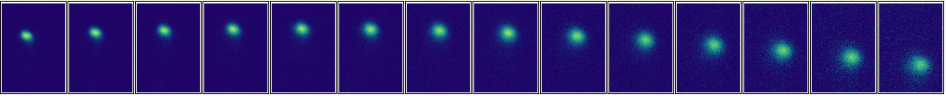
\includegraphics[width=0.8\textwidth]{molasses_launch}
    \caption[Atom cloud position after launching in a moving molasses]{A series of images showing the trajectory of the atom cloud after being cooled in a moving molasses. The first image was taken \sivalue{7}{\milli\second} after initiating the molasses and a subsequent one every \sivalue{5}{\milli\second}. Each image represents a region of interest of dimensions 1150 \(\times\) 1650 pixels that covers the spatial extent of the atom cloud during the launch.}
    \label{fig:molasses_launch}
\end{figure}
\subsubsection{Measuring the Temperature}
In thermal equilibrium, the velocity distribution of the atoms is described by a Maxwell-Boltzmann distribution
\begin{equation}
    f(v_x,v_y,v_z) = \left(\frac{m}{2\pi k_B }\right)^{3/2}e^{-\frac{m (v`_x^2+v`_y^2+v`_z^2)}{2 k_B T}}
    \label{eg:mb3D}
\end{equation}
where \(v`_i = v_i - \langle v_i \rangle\) is the difference from the average velocity. Along a single axis, the velocity distribution is obtained by integrating over the other velocity components. For the sake of notation, the following discussion uses \(x\) and \(v_x\) as labels for position and velocity, but these are interchangeable with the equivalent components along the other axes. As~\EquationRef{eg:mb3D} is a product of velocity distributions along each axis, the velocity distribution along one axis is 
\begin{equation}
    f(v_x) = \left(\frac{m}{2\pi k_B }\right)^{1/2}e^{-\frac{m (v_x-\langle v_x \rangle) ^2}{2 k_B T}}
    \label{eg:mb1D}
\end{equation}
Suppose that there are initially \(n_0 (x) \mathrm{d}x\) atoms within the region \((x, x+\mathrm{d}x)\), where \(n_0(x) = n(x, t=t_0)\) is the initial atomic density along one axis. During ballistic expansion, the atoms redestribute themselves according to their velocity. After a time \(t\) of free expansion, the position of an atom initially at \(x\) is \(x + v_x t\). 
Assuming that the number density is initially a Gaussian, with a peak number density \(n_0(x_0)\) at the centre-of-mass, the number density at later times is given by a convolution with~\EquationRef{eq:mb1D}
\begin{equation}
        n(x,t) = \int n_0(x_0) \left(\frac{m}{2\pi k_B}\right)^{1/2} e^{-\frac{m (v_x-\langle v_x \rangle)^2}{2 k_B T}} e^{-\frac{(x+v_x t - x_0)^2}{2\sigma_0^2}} \mathrm{d}v_x
        \label{eq:density_time}
\end{equation}
where \(\sigma_0\) is the \(1/e^2\) initial width of the cloud. As a convolution of two Gaussians, \EquationRef{eq:density_time} is also a Gaussian, with a \(1/e^2\) width given by
\begin{equation}
    \sigma(t)^2 = \sigma_0^2 + \frac{k_B T}{m} t^2
    \label{eq:expansion_width}
\end{equation}
\par\noindent
\FigureRef{fig:molasses_temperature} shows the measured cloud width over a range of expansion times. The inset shows a typical density profile along each axis, obtained by imaging the cloud on a camera, as previously described in~\SectionRef{eq:imaging}. For the purposes of measuring the temperature, the total atom number and the initial cloud size are not important, so no attempt was made to estimate these. The initial measurement was made \sivalue{7}{\milli\second} after the end of the molasses to allow for enough time to re-lock the laser to \(-0.5\Gamma\) below the \trans{2}{3} transition and align the bias field to the \(\vec{z}\) axis so that the atoms could be optically pumped into the \(\ket{2,2}\) state. At each measurement time, a non-linear least squares fit to~\EquationRef{eq:density_time} along each axis was carried out to estimate the width of the cloud. Then, a least squares linear fit was used to estimate the temperature along each axis from the gradient, as per~\EquationRef{eq:expansion_width}. The measured temperature along the horizontal and vertical axes of the camera was \(T_x = \sivalue{6.37 \pm0.15}{\micro\kelvin}\) and \(T_y = \sivalue{6.38\pm0.12}{\micro\kelvin}\), respectively.  

\begin{figure}
    \centering
    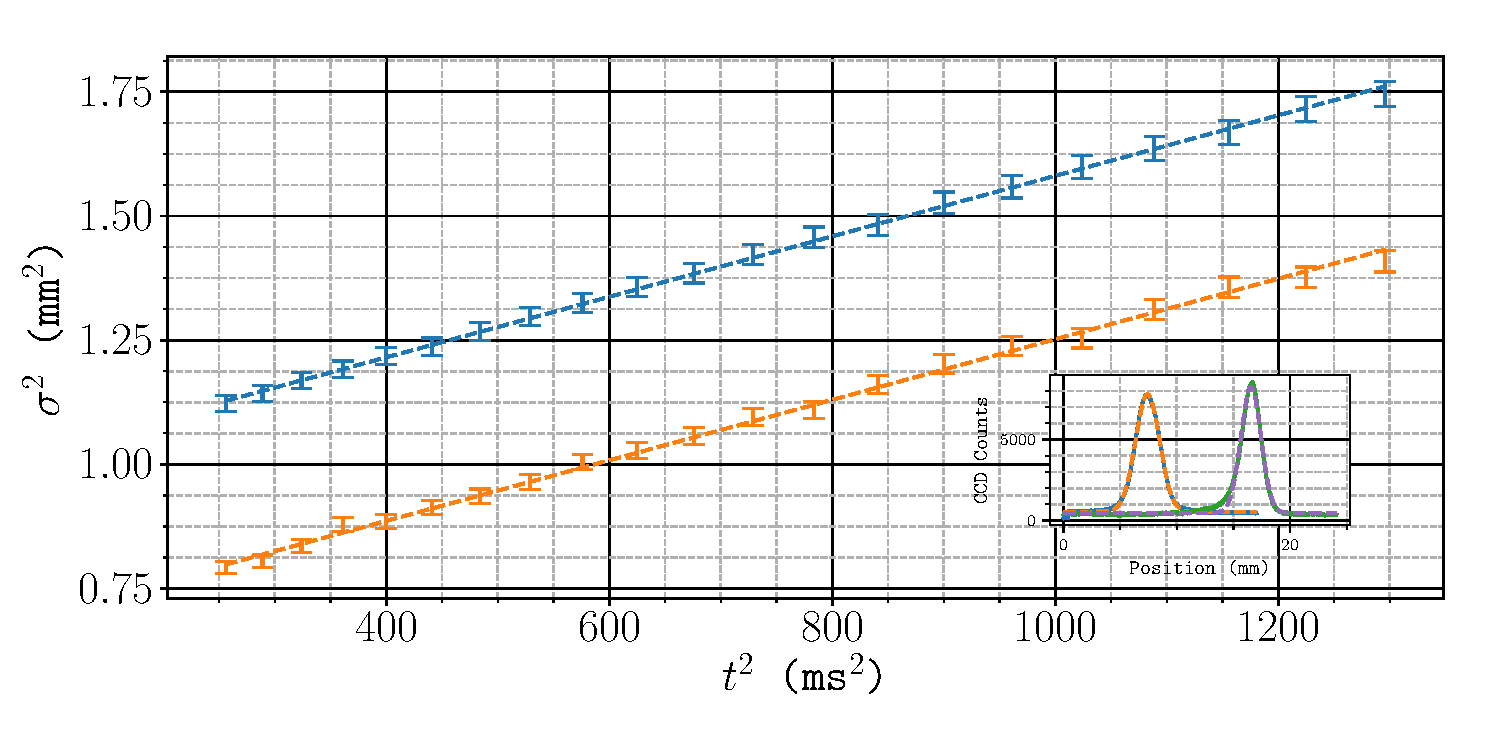
\includegraphics[width=0.8\textwidth]{temperature_launch}
    \caption[Temperature measurement using ballistic expansion]{Atom cloud temperature using a ballistic expansion measurement. After molasses, the cloud is left to expand in the dark and in a region of close to zero magnetic field. A least-squares linear fit of \(\sigma(t)^2\) is used to estimate the temperature using~\EquationRef{eg:expansion_width}. The inset shows a typical density profile from a single image, obtained by integrating the signal from a CCD camera along the two axes of the the sensor. The gradient from the fits for the horizontal (blue) and vertical (orange) axes are  \(T_x = \sivalue{6.38 \pm0.15}{\micro\kelvin}\) and \(T_y = \sivalue{6.38\pm0.12}{\micro\kelvin}\).}
    \label{fig:molasses_temperature}
\end{figure}

\subsubsection{Measuring the Launch Trajectory}
The same method used to measure the temperature of the cloud can also be used to measure the position of the centre-of-mass. In this case, the quantity of interest is \(\langle x(t)\rangle\). Since the cloud is in free-fall, the trajectory for the centre-of-mass is then given by the well-known equation-of-motion for a particle moving under constant acceleration
\begin{equation}
    \langle x(t) \rangle = \langle x(0) \rangle + v_x t + \frac{1}{2} a_x t^2
    \label{eq:position_free}
\end{equation}
where \(v_i\) is the initial velocity along the given axis and \(a_i\) is the acceleration.
\par\noindent
To launch the atoms both vertically and horizontally (along the axis parallel with the Raman light), the \((z_+, z_-)\) \acp{aoms} were ramped so that the relative frequency difference between each beam was \(2\times\)\sivalue{320}{\kilo\hertz} and the \(x\) and \(y\) \ac{aom} frequencies were ramped to give a frequency difference of \(2\times \sivalue{75}{\kilo\hertz}\) between the horizontal \ac{mot} beams. \FigureRef{fig:molasses_launch} is a plot of the measured centre-of-mass position along the horizontal and vertical camera axes over time. A linear least-squares fit to~\EquationRef{eq:position_free} gives a vertical launch quantities of \(v_v = \sivalue{25.0\pm0.35}{\centi\meter\per\second}\) and \(a_v = \sivalue{-9.40\pm0.075}{\metre\per\second\squared}\) and \(v_h = \sivalue{7.39\pm0.21}{\centi\meter\per\second}\) and \(a_h = \sivalue{-0.31\pm0.052}{\metre\per\second\squared}\) along the horizontal axis. 
\begin{figure}
    \centering
    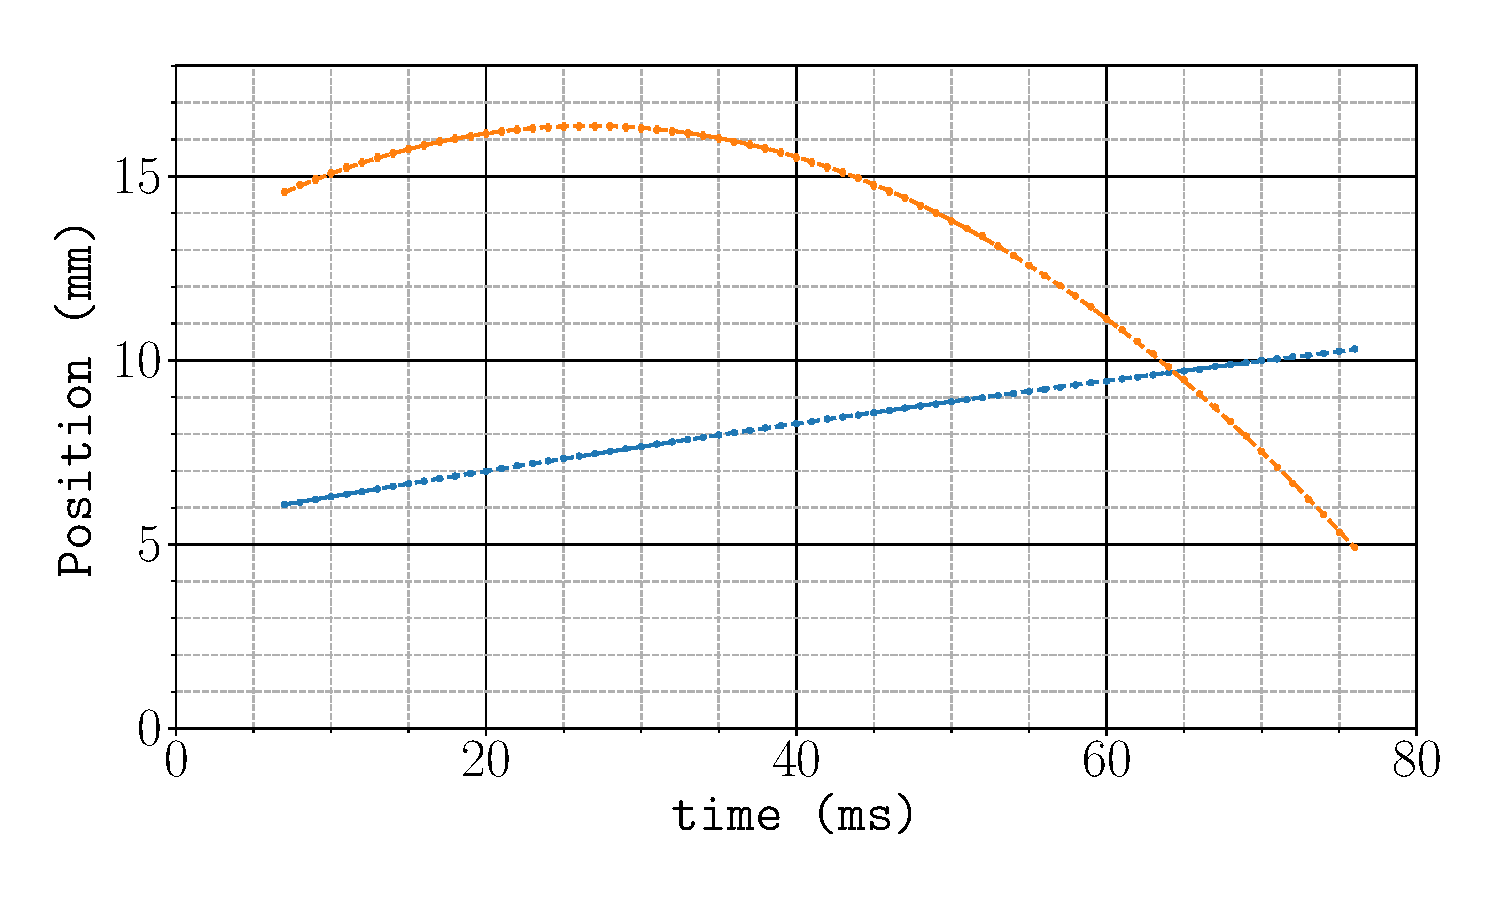
\includegraphics[width=0.8\textwidth]{molasses_position}
    \caption[Atom cloud centre-of-mass over time]{Measured centre-of-mass position over time. The horiztonal component of the position is shown in blue and the vertical in orange. Each trajectory is fit to~\EquationRef{eq:position_free} to estimate the launch velocity. The best-fit values are \(v_v = \sivalue{25.0\pm0.35}{\centi\meter\per\second}\) and \(a_v = \sivalue{-9.40\pm0.075}{\metre\per\second\squared}\) along the vertical axis and \(v_h = \sivalue{7.39\pm0.21}{\centi\meter\per\second}\) and \(a_h = \sivalue{-0.31\pm0.052}{\metre\per\second\squared}\) along the horizontal.}
    \label{fig:molasses_position}
\end{figure}
\par\noindent
When compared to the expected velocities from the detunings, \(v^{(l)}_v = \sivalue{24.96}{\centi\metre\per\second}\) and  \(v^{(l)}_h = \sivalue{5.85}{\centi\metre\per\second}\), the measured horizontal velocity is far greater than expected. This can be explained by a residual magnetic field, that is not cancelled using the bias coils. In the presence of a magnetic field, atoms cooled in an optical molasses are decelerated to a velocity at which the Zeeman shift is cancelled by the Doppler shift. This \ac{vsr} depends on the orientation of the magnetic field to the polarisation of the light. In a one-dimensional optical molasses, a {vsr} occurs at \(v_\text{res}^{(1)} = - \mu_B g_F B/\hbar k\) when the magnetic field is aligned with the wave-vector of the light \cite{VanderStraten1993}. When the field is aligned at an arbitrary angle an additional resonance at \(v_\text{res}^{(2)} = - \mu_B g_F B/2\hbar k\) is present, due to additional \(\left(\sigma^{\pm}-\pi\right)\) transitions~\cite{Chang2002}. A residual field along the Raman axis of \sivalue{20}{\milli\gauss} would shift the \ac{vsr} along \(\vec{x}\) and \(\vec{y}\) by \sivalue{1.09}{\centi\metre\per\second} corresponding to a velocity of \sivalue{1.54}{\centi\metre\per\second} along the Raman axis. 

\section{State Preparation}\label{sec:state_prep}
After the atoms have been cooled in an optical molasses, the population will mostly be distributed across the \(\ket{F=2}\) level, along with a small fraction distributed across the \(\ket{F=1}\) level. The Raman transition only couples the \(\ket{1,0}\) and \(\ket{2,0}\) states, so atoms in the other hyperfine ground states cannot participate in the interferometer. In fact, since the individual Zeeman sub-levels are not resolved during detection, these background atoms result in a loss of fringe visibility. One way to overcome this is to apply a pulse of light resonant with the \trans{2}{3} transition to push the non-participating atoms out of the interferometer detection region. Of course, this must be done after applying a Raman pulse to transfer an ensemble of atoms from \(\ket{2,0}\) into \(\ket{1,0}\). In this simple scheme a large fraction of the atoms are removed, which is undesirable since measurements of a low number of atoms are inherently more uncertain due to shot number fluctuations. 
\par\noindent
The following section discusses a method of preparing the atoms to increase the population in the \(\ket{1,0}\) ground state. An overview of the scheme is given in~\SectionRef{subsec:prep_schemes}. This is followed by a discussion of the initial steps which optically pump atoms into the \(\ket{1,0}\) state in~\SectionRef{subsec:optical_pumping}. A description of the microwave pulse used to drive atoms into the \(\ket{F=2}\) level is given in~\SectionRef{subsex:microwaves}. This section concludes with the method used to blow away the atoms which do not contribute to the interferometer in~\SectionRef{subsec:blow_away}. A key step which has been omitted is the velocity-selective Raman pulse. This is described in more detail later, in~\SectionRef{subsec:raman_velocity_select}
\subsection{Schemes for Preparation}\label{subsec:prep_schemes}
The scheme used to prepare atoms in the \(\ket{1,0}\) state is the following:
\begin{enumerate}
    \item Light resonant with the \trans{2}{2} transition pumps atoms into the \(\ket{F=1}\) level
    \item Light resonant with the \trans{1}{0} transition drives (\(\sigma^{\pm}\)) transtions to pump atoms into the \(\ket{1,0}\) dark state
    \item A microwave $\pi$-pulse transfers atoms to \(\ket{2,0}\)
    \item A Raman $\pi$-pulse transfers atoms with a narrow velocity spread back to \(\ket{1,0}\)
    \item The atoms which remain in \(\ket{F=2}\) are blown away
\end{enumerate}
A diagram of the population of each hyperfine ground state and the laser frequencies used to drive these transitions is given in~\FigureRef{fig:state_prep}. With the exception of step 4, the light is provided by the \Muquans laser using the \ac{mot} collimators aligned to the vertical \(\vec{z}\) axis. The frequency of the cooling laser and the repump sideband are set so that the relevant transitions for steps 1 and 2 are addressed. As the \(\ket{F=1}\) light is a sideband of the \(\ket{F=2}\) light, it is not possible to blow away atoms in \(\ket{F=1}\) without also blowing away atoms in \(\ket{F=2}\). This problem is overcome by using microwave pulses to drive atoms up to \(\ket{F=2}\) before velocity selection.
\par\noindent
A timing diagram of the state preparation sequence is shown in~\FigureRef{fig:state_selection_timing}, which indicates the duration for which each optical or microwave pulse is applied, as well as the direction of the applied magnetic field. The field is switched slowly over \sivalue{2}{\milli\second} (which is omitted from the diagram) to preserve the spin state of each atom. 
\begin{figure}
    \centering
    %\def\svgwidth{0.8\textwidth}
    \fontsize{16pt}{16pt}
    \resizebox{0.8\textwidth}{!}{\input{state_selection.pdf_tex}}
    \caption[State preparation pulse sequence]{Sequence of optical and microwave pulses used to prepare an ensmble of atoms in \(\ket{1,0}\). The red arrows indicate optical transitions to and from \(\ket{F=2}\) and equivalently for the blue arrows and \(\ket{F=1}\). A residual population in the \(\ket{1,\pm 1}\) states is present, which contributes to a background during the interferometer.}
    \label{fig:state_prep}
\end{figure}
\begin{figure}
    \centering
    %\def\svgwidth{0.5\textwidth}
    \fontsize{14pt}{14pt}
    \resizebox{0.6\textwidth}{!}{\input{state_selection_timing.pdf_tex}}
    \caption[State selection timing schematic]{Timing diagram for state selection sequence. The durations labelled are indicative of the time required to drive the atoms into the desired state at each step. After the \trans{1}{0} pumping, the magnetic field is re-oriented along the Raman axis \(\vec{r}\). The \sivalue{2}{\milli\second} field switching time has been omitted.}
    \label{fig:state_selection_timing}
\end{figure}
\subsection{Optically Pumping the Atoms}\label{subsec:optical_pumping}
\subsubsection{Driving the \trans{2}{2} transition}
After the molasses, the frequency of cooling light is \sivalue{150}{\mega\hertz} below the \trans{2}{3} transition. This can off-resonantly excite an atom to the \(\ket{F'=2}\) excited level, but the small scattering rate means that on average, an atom will need to scatter many photons before it is pumped into the \(\ket{F=1}\) level. Therefore, to minimise the heating during this pumping process, the frequency of the cooling light is resonant with the \trans{2}{2} transition.
\par\noindent
\FigureRef{fig:step1_pumping} shows the population in the two hyperfine ground states as the duration of the \trans{2}{2} light is increased. The rate at which atoms are pumped into \(\ket{F=1}\) increases with the strength of the applied magnetic field. At zero field, there exists a dark state which is a coherent superposition of the \(\ket{2,m_F}\) states~\cite{Berkeland2002}. Applying a magnetic field lifts the degeneracy between the Zeeman sub-levels so that this dark state is no longer stationary. The evolution rate of this dark state, and hence pumping rate, increases with an increasing Zeeman shift. At a field strength of \sivalue{3}{\gauss}, the atoms can be pumped into \(\ket{F=1}\) in less than \sivalue{5}{\micro\second}.
\begin{figure}
    \centering
    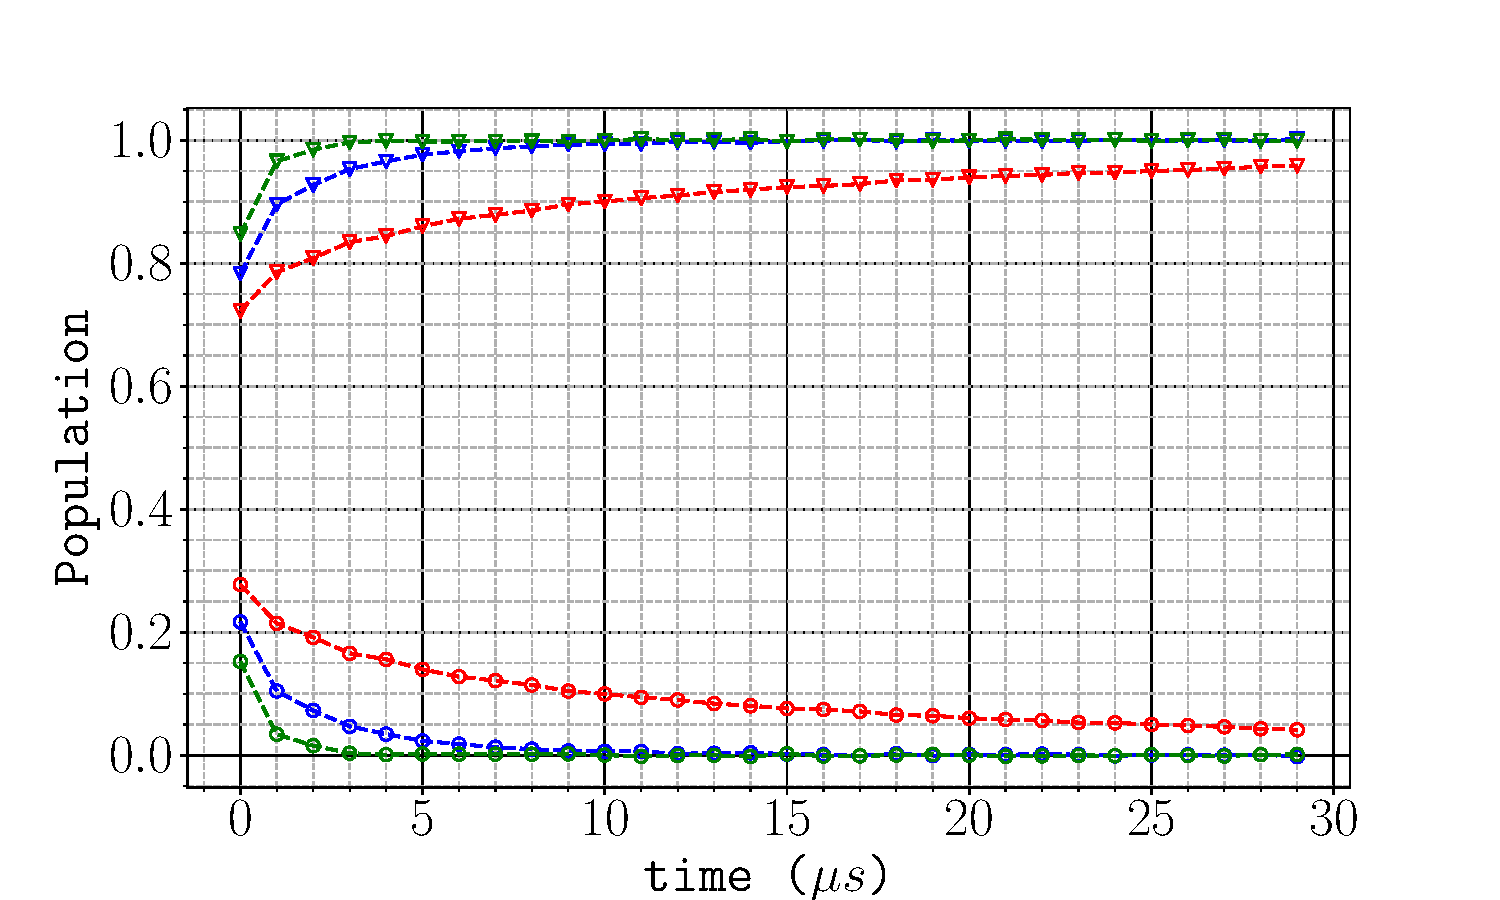
\includegraphics[width=0.5\textwidth]{step1_pumping}
    \caption[Ground state distribution during \trans{2}{2} pumping]{Population across the two hyperfine ground states after \trans{2}{2} pumping under various magnetic field strengths. The $\smalltriangledown$ ($\circ$) markers indicate the population in $\ket{F=2}$ ($\ket{F=1})$. The red, blue and green series correspond to field strengths of \sivalue{-0.16}{\gauss}, \sivalue{1.67}{\gauss}, and \sivalue{3}{\gauss}, respectively.}
    \label{fig:step1_pumping}
\end{figure}
\subsubsection{Driving the \trans{1}{0} transition}
After this first pumping step, the atoms are distributed across the Zeeman sub-levels in \(\ket{F=1}\). The next pulse of light is used to increase the population in \(\ket{1,0}\) by driving \trans{1}{0} transitions. During this time, the \trans{2}{2} light remains on which helps to prevent atoms from populating the \(\ket{F=2}\) level through off-resonant \trans{1}{1} excitations. The magnetic field present means that the circularly-polarised \(\vec{z}\) \ac{mot} beams only drive \(\sigma^{\pm}\) transitions, so the \(\ket{1,0}\) state is in principle a dark state. 
\par\noindent
The distribution of atoms across the Zeeman sublevels was measured using a microwave pulse to drive atoms into the \(\ket{F=2}\) level, which is described in~\SectionRef{subsec:microwaves}. For each \(\pi\) microwave transition, the frequency of the microwave field was varied to find the resonant frequency. The resulting spectra for \(m_F = -1\)  and \(m_F = 0\) are shown in~\FigureRef{fig:step2_microwave_spec}, both with and without applying light to pump into the \(\ket{1,0}\) state.  The 0 \(\rightarrow\) 0 clock transition is detuned from the hyperfine splitting frequency due to the applied magnetic field, giving a second-order Zeeman shift of \sivalue{515}{\hertz\per\gauss\squared}. The measured shift of \sivalue{5.6}{\kilo\hertz} corresponds to a field strength of \sivalue{3.3}{\gauss}.
\begin{figure}
    \centering
    \def\svgwidth{\columnwidth}
    \subfloat[][]{\scalebox{0.3}{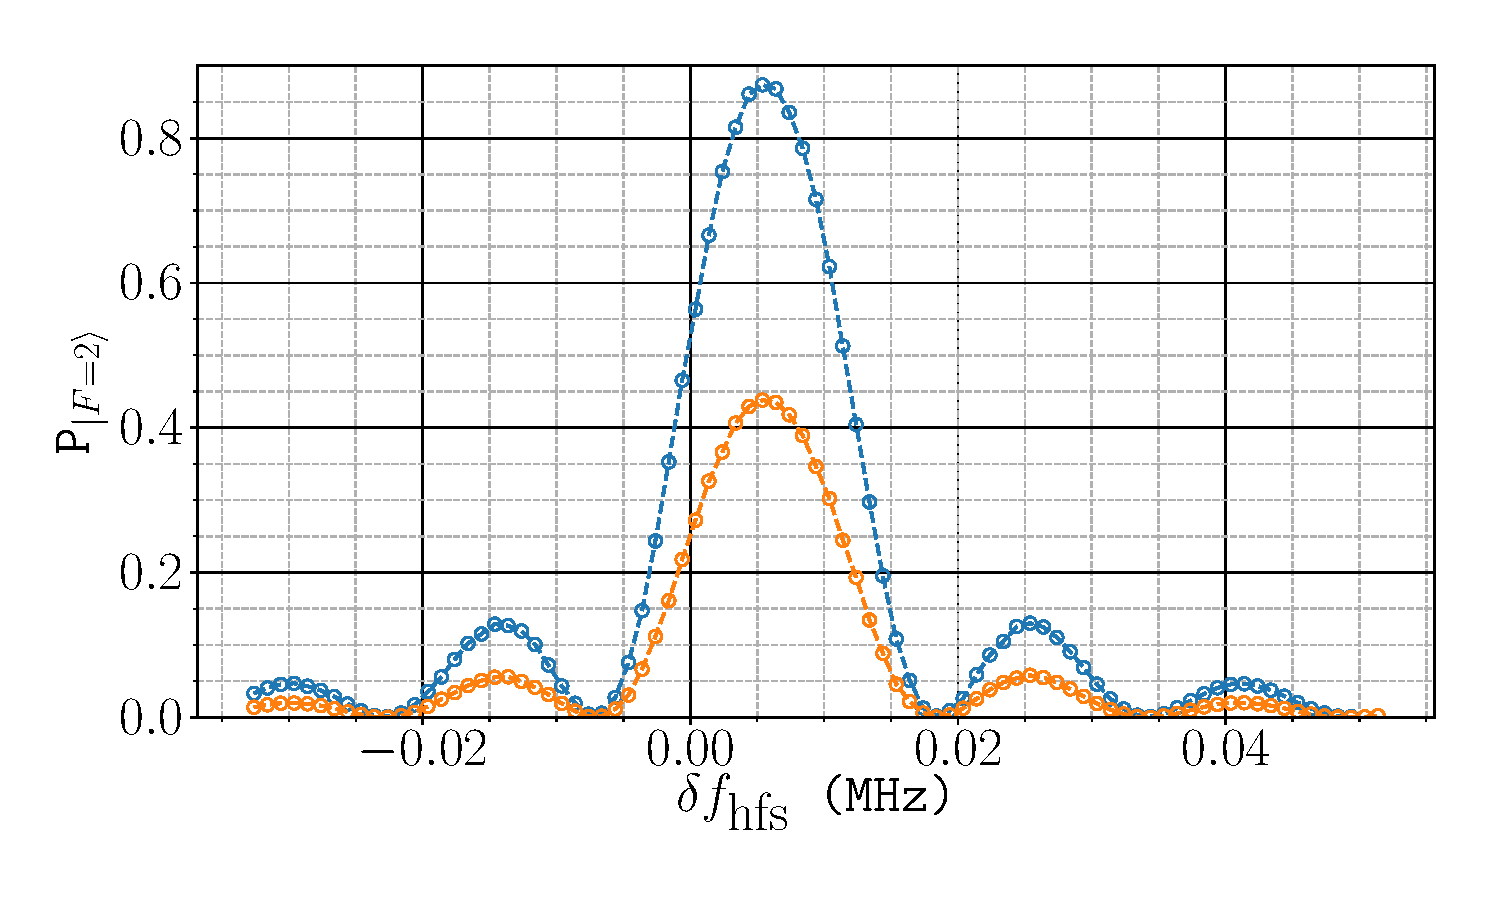
\includegraphics{step2_mf0}}\label{fig:step2_mf0}}
    \subfloat[][]{\scalebox{0.3}{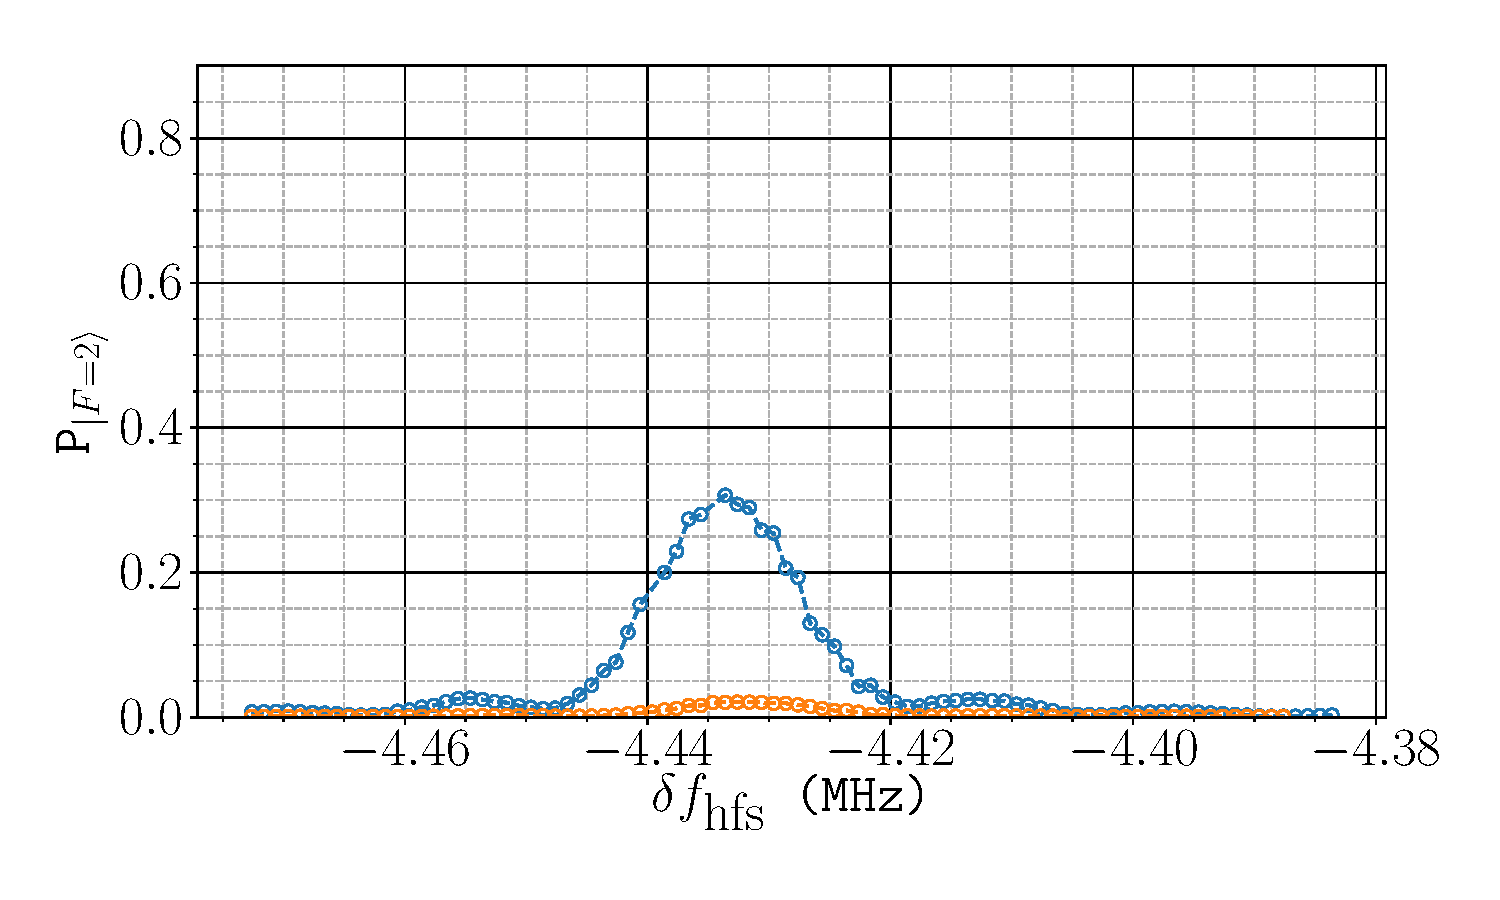
\includegraphics{step2_mf1}}\label{fig:step2_mf1}}
    \caption[\(m_F\) populations before and after \trans{1}{0} pumping]{Population of atoms in (a) \(\ket{1,0}\) and (b) \(\ket{1,-1}\), measured by applying a \sivalue{68}{\micro\second} microwave pulse to drive atoms into the \(\ket{F=2}\) level. The orange and blue points indicate the measured populations with and without \trans{1}{0} pumping. The microwave frequency is plotted as a detuning from the hyperfine splitting frequency \(f_\text{hfs}\).}
    \label{fig:step2_microwave_spec}
\end{figure} 
\par\noindent
A plot of the population in each Zeeman sub-level for increasing pumping times is given in~\FigureRef{fig:step2_pumping}. In this instance, the optical pumping does not completely deplete the population from the \(m_F = \pm 1\) sub-levels. After pumping for \sivalue{30}{\micro\second}, approximately 5\% of the population remains in the \(m_F = \pm 1\) sub-levels. The \(\ket{1,0}\) state can only be excited to \(\ket{F'=0}\) by \(\pi\)-polarised light, which suggests that the magnetic field is mis-aligned with the \(\vec{z}\) \ac{mot} beams. The effect of these background atoms on the measured interferometer signal is discussed later, in~\SectionRef{subsec:phase_measurement}.
\begin{figure}
    \centering
    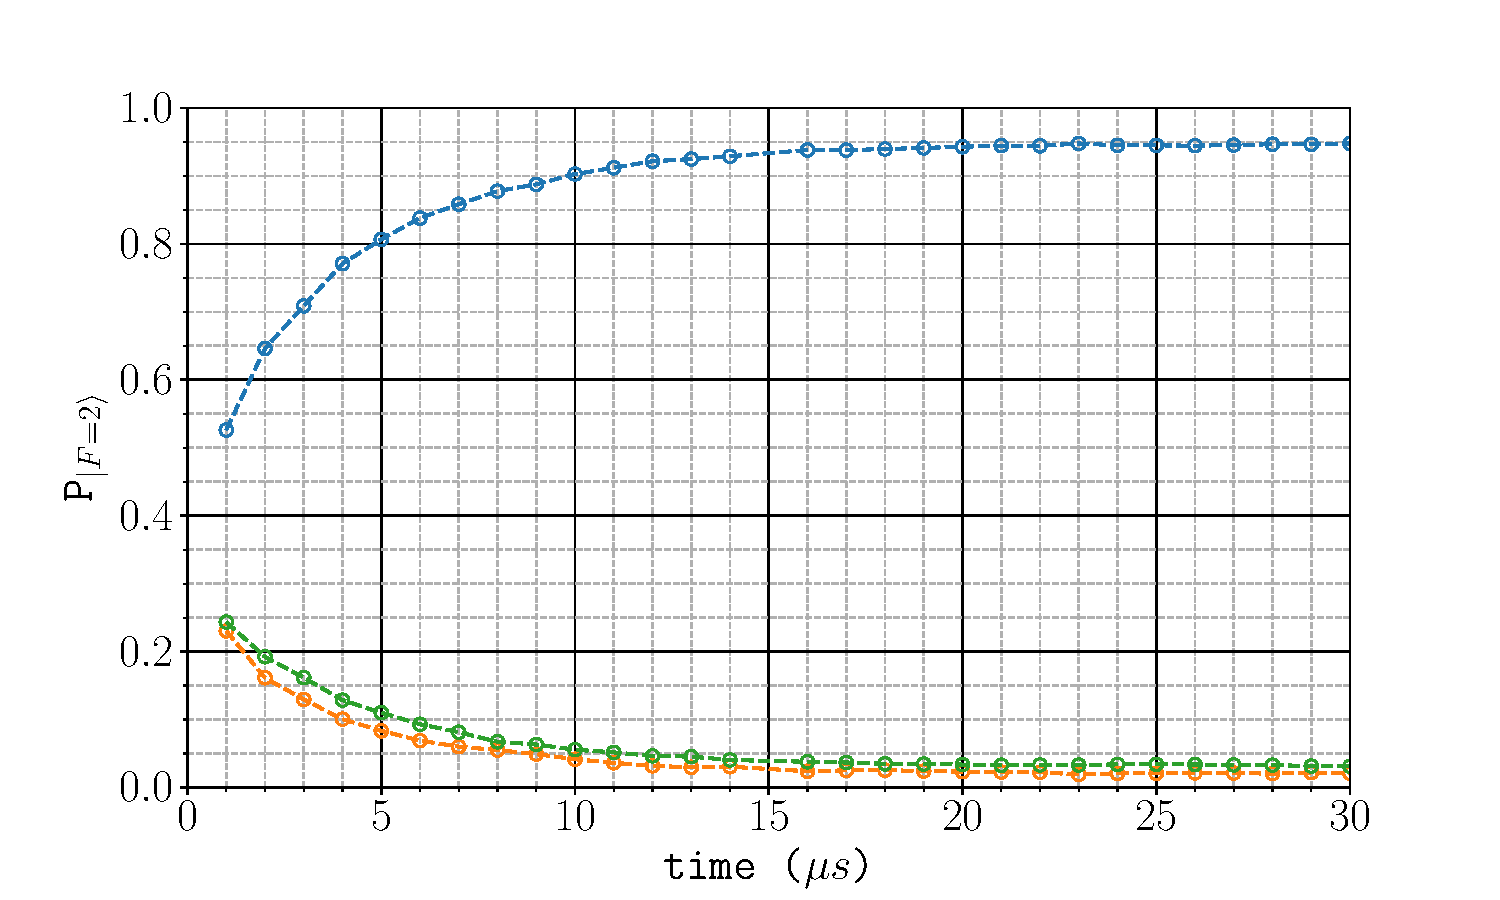
\includegraphics[width=0.8\textwidth]{step2_pumping}
    \caption[\(\ket{1,m_F}\) populations for increasing \trans{1}{0} pumping time.]{Population in each Zeeman sub-level as the \trans{1}{0} pumping time is increased. The \(m_F = 0, -1, +1\) populations are shown in blue, orange and green, respectively. After \sivalue{30}{\micro\second}, approximately 5\% of the population remains in the \(m_F = \pm 1\) sub-levels.}
    \label{fig:step2_pumping}
\end{figure}
\subsection{Including Microwave Transitions}\label{subsec:microwaves}
Without a dedicated laser to drive transitions from the \(\ket{F=1}\) level, it was necessary to implement a scheme to use light resonant with the \(\ket{F=2}\) level to remove background atoms. Therefore, we included a system for driving microwave frequency transitions from \(\ket{1,0}\) to \(\ket{2,0}\).
\subsubsection{Microwave Generation}
A diagram of the setup for this is shown in~\FigureRef{fig:microwave_setup}. The microwave radiation is generated using a \textit{Wind-Freak} synthesiser to output a microwave field oscillating at a frequency close to the hyperfine splitting frequency, \(f_\text{hfs} = \sivalue{6.83846}{\giga\hertz}\). This is amplified by \textit{MiniCircuits MCL ZRON-8G+} amplifier and directed into the chamber using a \textit{Pasternack PE9859/SF-10} microwave horn, which produces a linearly-polarised microwave field. The horn was aligned to the chamber at the position which maximised the population of atoms in the \(\ket{2,0}\) state. The synthesiser is clocked using a stable \sivalue{100}{\mega\hertz} signal from the \Muquans laser. When the synthesiser was clocked using its internal \sivalue{27}{\mega\hertz} reference clock, this produced a noticeable jitter in the output frequency, which led to a significant shot-to-shot fluctuation in the \(\ket{2,0}\) population.
\begin{figure}
    \centering
    \resizebox{0.5\textwidth}{!}{\input{microwave_setup.pdf_tex}}
    \caption[Setup for Microwaves]{Schematic diagram of the microwave assembly. The frequency close to the hyperfine splitting frequency is generated by a \textit{Wind-Freak} synthesiser. A \sivalue{100}{\mega\hertz} clock signal acts as a stable reference frequency for the synthesiser. The generated microwave power is amplified twice, first by a low-power \textit{Mini-Circuits} amplifier, then by a microwave horn, which produces a highly directional, linearly polarised wave. The output is controlled by a digital signal, both at the synthesiser and at a bi-directional microwave switch. The second port of this is blocked with a \sivalue{50}{\ohm} terminator to prevent reflections. }
    \label{fig:microwave_setup}
\end{figure}
\subsubsection{Pulse Characterisation}
\FigureRef{fig:mw_rabi} shows a measurement of the population in the \(\ket{F=2}\) level for increasing durations duration of the applied microwave pulse. Rabi oscillations between the \(\ket{1,0}\) and \(\ket{2,0}\) states are clearly present. The loss of coherence between the states can be explained by an inhomogeneous driving field. Once inside the chamber, the microwaves reflect and scatter off the interior surfaces which results in a spatially-dependent Rabi frequency. This also leads to a depolarisation of the field, as \(\sigma^{\pm}\) transitions were also observed. Initially, around \(85\%\) of the population was driven into \(\ket{F=2}\) using a microwave pulse of \sivalue{100}{\micro\second}. After improving the alignment of the magnetic field during the microwave pulse, this fraction increased to \(97\%\) - the remaining 3\% being distributed across the \(m_F = \pm 1\) states.

\begin{figure}
    \centering
    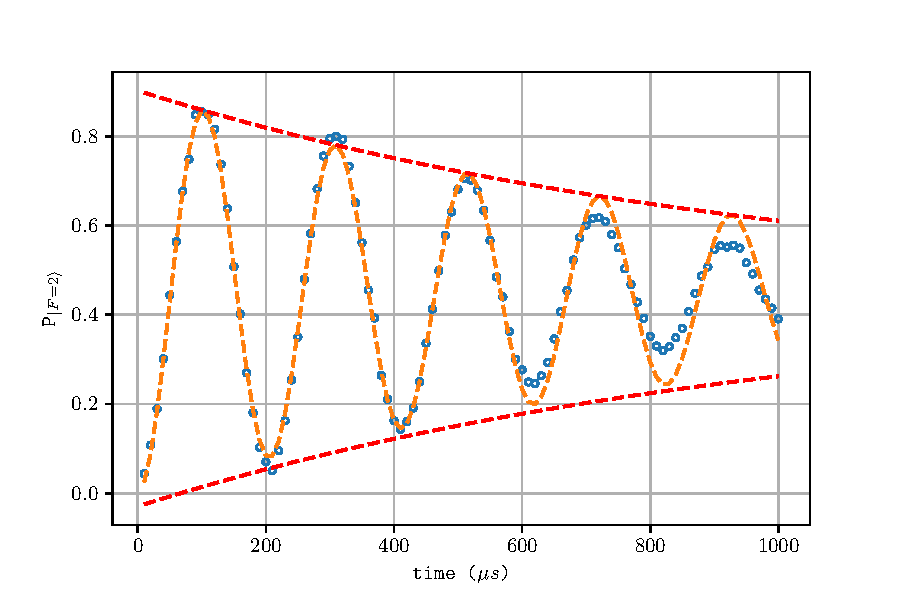
\includegraphics[width=0.5\textwidth]{mw_rabi}
    \caption[Microwave Rabi oscillation between \(\ket{1,0}\) and \(\ket{2,0}\)]{Damped Rabi oscillation between \(\ket{1,0}\) and \(\ket{2,0}\) using a microwave pulse of varying length. At longer pulse times, there is a loss of coherence due to a depahasing between the two states. The red dashed line is an envelope is a fit to a decaying exponential with a characteristic time of \(\tau = \sivalue{1016}{\micro\second}\).}
    \label{fig:mw_rabi}
\end{figure}
\par\noindent
\FigureRef{fig:microwave_transitions} shows a spectrum obtained by varying the frequency of the microwave pulse. This shows the presence of \(\Delta m = \pm 1 \) transitions from \(\ket{1,0}\), as well as the fact that the population in \(\ket{1,m_F=\pm 1}\) decreases after the \trans{1}{0} pumping step is applied. The linewidth of the microwave transition is much narrower than the Zeeman splitting, so only the clock transition is driven when a pulse with a frequency close to \(f_\text{hfs}\) is applied.
\begin{figure}
    \centering
    \def\svgwidth{\columnwidth}
    \subfloat[][]{\scalebox{0.7}{\input{microwave_spectrum.pdf_tex}}\label{fig:microwave_spectrum}}
    \subfloat[][]{\scalebox{0.3}{\raisebox{3ex}{\input{microwave_transitions.pdf_tex}}}}
    \caption[Microwave transition spectrum]{Microwave transition spectrum before (blue) and after (orange) \trans{1}{0} pumping. (b) shows the transitions addressed as the microwave frequency is varied. Dashed and lines indicate \(\Delta m = \pm 1\) transitions and solid lines indicate \(\Delta m = 0\). In order of increasing frequency, the transitions in (a) are highlighted in: a) red, b) blue, c) green, d) orange and e) purple.} 
    \label{fig:microwave_data}'
\end{figure}

\subsection{Blow-Away}\label{subsec:blow_away}
After the atoms populate \(\ket{2,0}\), a velocity-selective Raman \(\pi\)-pulse is applied to transfer a fraction of those back into \(\ket{1,0}\). This step is discussed in detail in~\SectionRef{subsec:raman_velocity_select}. For now, it suffices to say that a Raman pulse transfers 4\% \textbf{Check this!} the atoms back to \(\ket{1,0}\). The remaining need to be removed, otherwise they contribute to a large background signal. \par\noindent
The final pulse during the state preparation sequence is used to push these non-contributing atoms out of the interferometer region. A single \ac{mot} beam is used so that there is a net momentum transfer to the atoms as they absorb light and fluoresce. The frequency of this blow-away beam is detuned from the \trans{2}{3} transition by \sivalue{-3}{\mega\hertz}, which is the same frequency used for detection (see~\SectionRef{sec:atom_detection}). A pulse of \sivalue{50}{\micro\second} is enough to remove all atoms in \(\ket{F=2}\). 

% \subsection{Residual \(m_F = \pm 1\) atoms} \label{subsec:residual_atoms}
% After preparing an ensemble atoms in \(\ket{1,0}\) with a narrow velocity spread and removing those out in \(\ket{F=2}\) which are not resonant with the interferometer pulses, there is still a fraction of atoms in \(\ket{1,\pm 1}\) which will be detected and contribute to a background signal. It is worth highlighting how fluctuations in this background affects the sensitivity of the interferometer to accelerations. Since they are not driven by the Raman transition, they remain in \(\ket{F=1}\). If the number of atoms detected in \(\ket{F=1}\) has a contribution from background atoms, i.e \(N_1 = N_\text{bg}+N_1^{(\phi)}\), then the probability of detecting an atom in \(\ket{F=1}\) is given by
% \begin{equation}
%     P_{\ket{F=1}} = P_0 + \frac{C}{2}\sin{\Delta \phi}^2
% \end{equation}
% where \(P_0 = N_\text{bg}/\left(N_1+N_2\right)\) is the proportion of background atoms out of the total number of atoms.

\subsection{Conclusion}
This chapter has presented the stages of the experiment which are used to prepare an ensemble of atoms for interferometry. This requires cooling the atoms to limit the thermal expansion of the cloud during interferometry. The atoms are also launched using a moving molasses so that only one pair of beams is resonant with the Raman transition. Finally, we then apply a sequence of optical and microwave pulses, to increase the population of atoms in \(\ket{1,0}\). A velocity-selective Raman pulse with a narorow linewidth is used to make the velocity spread along the Raman axis much smaller than the Doppler width. Aside from some residual population in \(\ket{1,\pm 1}\), the remaining atoms are removed using a pulse of light close to resonance with the \trans{2}{3} transition. This results in an ensemble of which around \(40\%\) of the population contributes to the interferometer signal.

